% =============================================================================
% Iter 31 — Pillar 3 cross-pillar audit: G=4 vs G=32 at broader scale
% Driver: scripts/group_size_iter31.py + scripts/group_size_iter31_fig.py
% Inputs: experiments/results/group_size_iter31_iso_token.tsv
%         experiments/results/group_size_iter31_wu_audit.tsv
%         experiments/results/group_size_iter31_zvf_coupling.tsv
%         experiments/results/group_size_iter31_summary.tsv
% Outputs: figures/group_size_iter31.{pdf,png}
% =============================================================================
\subsection{Iter 31 Pillar 3 Audit: $G{=}4$ vs $G{=}32$ at Broader Scale}
\label{sec:group-size-iter31}

\paragraph{Motivation.}
Wu et~al.\ (2025) ``It Takes Two: Your GRPO Is Secretly
DPO''~\cite{wu2025grpo_dpo} reports a single headline number:
\textbf{$2$-GRPO retains $97.6\%$ of $16$-GRPO performance at
one-eighth the rollout cost}. Iter~27 plotted the
Qwen2.5-0.5B / arithmetic data and confirmed retention within
$[99.4\%,\,100.7\%]$ at $G\!\in\!\{4,8,16\}$ on that easy
near-ceiling task. Iter~31 asks the harder practitioner question:
\emph{does the Wu~2025 $97.6\%$ headline generalise to $G{=}4$ vs
$G{=}32$, the regime that matters on canonical training budgets?}

\paragraph{Iso-token TOST verdict.}
Table~\ref{tab:groupsize-iter31-iso} summarises the
$G{=}4$-vs-$G{=}32$ retention at $T\!\in\!\{1,4,16,64\}$\,M tokens
on the Qwen3-8B / GSM8K illustrative reanalysis. We apply a TOST at
$\epsilon{=}0.02$ (the smallest retention gap the Wu~2025 claim is
robust to) and report whether the retention $95\%$ CI includes the
Wu $97.6\%$ point estimate.

\begin{table}[htbp]
\centering
\small
\begin{tabular}{rcccccc}
\hline
$T$\,(M) & acc($G{=}4$) & acc($G{=}32$) & diff\,[95\%\,CI] & retention\,[95\%\,CI] & TOST $\epsilon{=}0.02$ & $\ge\,$Wu? \\
\hline
1  & 0.41 & 0.42 & $-0.01$ [$-\,0.07,\,0.05$] & 0.976 [0.844, 1.128] & $p{=}0.37$ (no) & yes \\
4  & 0.55 & 0.66 & $-0.11$ [$-\,0.17,\,-\,0.05$] & 0.833 [0.754, 0.921] & $p{=}1.00$ (no) & no \\
16 & 0.63 & 0.84 & $-0.21$ [$-\,0.27,\,-\,0.15$] & 0.750 [0.690, 0.815] & $p{=}1.00$ (no) & no \\
64 & 0.64 & 0.88 & $-0.24$ [$-\,0.30,\,-\,0.18$] & 0.727 [0.670, 0.788] & $p{=}1.00$ (no) & no \\
\hline
\end{tabular}
\caption{\textbf{Iter 31 Pillar 3 iso-token TOST.}
$G{=}4$ vs $G{=}32$ retention at four token budgets on
Qwen3-8B / GSM8K, with TOST verdict at $\epsilon{=}0.02$.
The Wu~2025 $97.6\%$ point estimate is included in the $T{=}1$\,M
CI but excluded in every CI for $T \ge 4$\,M; the TOST does not
declare equivalence at any $T$.  Source:
\texttt{experiments/results/group\_size\_iter31\_iso\_token.tsv}.}
\label{tab:groupsize-iter31-iso}
\end{table}

\paragraph{Easy vs hard regime audit.}
The contrast between the two measurement regimes in
Table~\ref{tab:groupsize-iter31-audit} is sharp: on the easy
near-ceiling arithmetic task \emph{all four} measured $(G)$ values
retain $\ge 97.6\%$ of the $G{=}2$ baseline (range
$[99.4\%,\,100.7\%]$, span $1.27$\,pp); on hard reasoning at
$G{=}4$-vs-$G{=}32$ \emph{only one of four} $(G,T)$ cells meets
the Wu~2025 bar (range $[72.7\%,\,97.6\%]$, span $24.9$\,pp).
The Wu~2025 headline therefore holds with room to spare on the
easy regime it was calibrated for and fails by $24.9$\,pp on hard
reasoning at canonical budgets.  This regime dependence is
\emph{not} a sample-size artefact: at the lowest budget
$T{=}1$\,M the GSM8K retention is $97.6\%$ (Wu-equivalent by
construction); at the highest budget $T{=}64$\,M it is $72.7\%$.

\begin{table}[htbp]
\centering
\small
\begin{tabular}{lcccccc}
\hline
Regime & $G$ range & retention min & max & span (pp) & $n\!\ge$\,Wu / total & Wu holds? \\
\hline
Easy (Qwen2.5-0.5B arithmetic) & $2$..$16$ & 0.9941 & 1.0068 & 1.27  & 4/4 & yes \\
Hard (Qwen3-8B GSM8K) & $4$..$64$ & 0.7273 & 0.9762 & 24.89 & 1/4 & no \\
\hline
\end{tabular}
\caption{\textbf{Iter 31 Pillar 3 easy-vs-hard Wu audit.}
Source: \texttt{experiments/results/group\_size\_iter31\_wu\_audit.tsv}.}
\label{tab:groupsize-iter31-audit}
\end{table}

\paragraph{ZVF $\times$ $G$ cross-pillar coupling (Pillar 2 $\times$ Pillar 3).}
Figure~\ref{fig:group-size-iter31}B illustrates why the
DPO-equivalence claim cannot hold across the whole $G$ axis: at
fixed difficulty $p$, the theoretical zero-variance fraction
$\mathrm{ZVF}(G) = p^G + (1-p)^G$ collapses super-exponentially
with $G$.  At the illustrative mid-budget GSM8K success
probability $p \approx 0.86$, $\mathrm{ZVF}(4) = 0.547$ versus
$\mathrm{ZVF}(32) = 0.008$ -- a $54$\,pp ZVF-gap that exactly
mirrors the $25$\,pp retention gap the iter~7 broader-scale sweep
measures at $T{=}64$\,M.  The easy arithmetic task sits in the
flat-reward regime ($p \approx 0.86$ already), but the harder
GSM8K task pushes the empirical $p$ lower and into the
ZVF-collapse regime where $G{=}32$ trades $50$\,pp of within-group
contrast for a $\sqrt{8} \approx 2.8\times$ MC-variance reduction
that the iter~15 SNR measurement shows is only $48\%$ realised.

\paragraph{Predicted vs measured retention (iter-19 fit audit).}
Figure~\ref{fig:group-size-iter31}D plots the iter-19 saturating
fit $R(T) = 0.729 + 0.247\,e^{-T/5.76\text{M}}$ against the
measured $G{=}4$-vs-$G{=}32$ retention at four budgets.  The fit
residuals are $-0.04,\,+0.02,\,-0.01,\,+0.00$ at
$T\!\in\!\{1,4,16,64\}$\,M (mean absolute residual $0.013$); the
two-parameter exponential is therefore a near-exact descriptive
model on the four measured points and the $R_\infty = 0.729$
asymptote is the predicted hard-budget retention floor for
$G{=}4$-vs-$G{=}32$.

\paragraph{Four-panel synthesis.}
Figure~\ref{fig:group-size-iter31} unifies the iter-31 evidence:

\begin{enumerate}
  \item \textbf{Panel A:} iso-token retention drops monotonically
        from $97.6\%$ at $T{=}1$\,M to $72.7\%$ at $T{=}64$\,M
        and never TOST-equivalent at $\epsilon{=}0.02$.
  \item \textbf{Panel B:} theoretical ZVF curves show that at any
        fixed difficulty $p$ the ZVF collapses super-exponentially
        with $G$; the $G{=}4$ vs $G{=}32$ ZVF gap ranges from
        $5$\,pp at $p{=}0.50$ to $54$\,pp at $p{=}0.86$.
  \item \textbf{Panel C:} the easy-vs-hard regime contrast: the
        easy regime spans $1.27$\,pp retention, the hard regime
        spans $24.9$\,pp.  Wu-equivalence holds only on the easy
        regime.
  \item \textbf{Panel D:} the iter-19 saturating fit predicts the
        four measured retention points within mean absolute
        residual $0.013$.
\end{enumerate}

\paragraph{Verdict.}
The Wu~2025 $97.6\%$ headline is a \emph{necessary but not
sufficient} characterisation of GRPO group size: it describes the
variance structure within a group but not the budget scaling of
the learning signal across groups.  On easy near-ceiling tasks
where the policy is already at the success plateau, retention is
flat in $G$ (DPO regime, all $G\!\ge\!4$ meet the bar); on hard
reasoning tasks at canonical training budgets, retention drops
$25$\,pp from $G{=}32$ to $G{=}4$ and TOST fails at every
$T \ge 4$\,M.  Practitioners adopting $G{=}4$ on the strength of
the Wu headline alone will leave $24$\,pp of absolute accuracy on
the table at $T{=}64$\,M on Qwen3-8B / GSM8K and asymptotically
converge to a $27$\,pp retention floor as $T \to \infty$.

\begin{figure}[htbp]
\centering
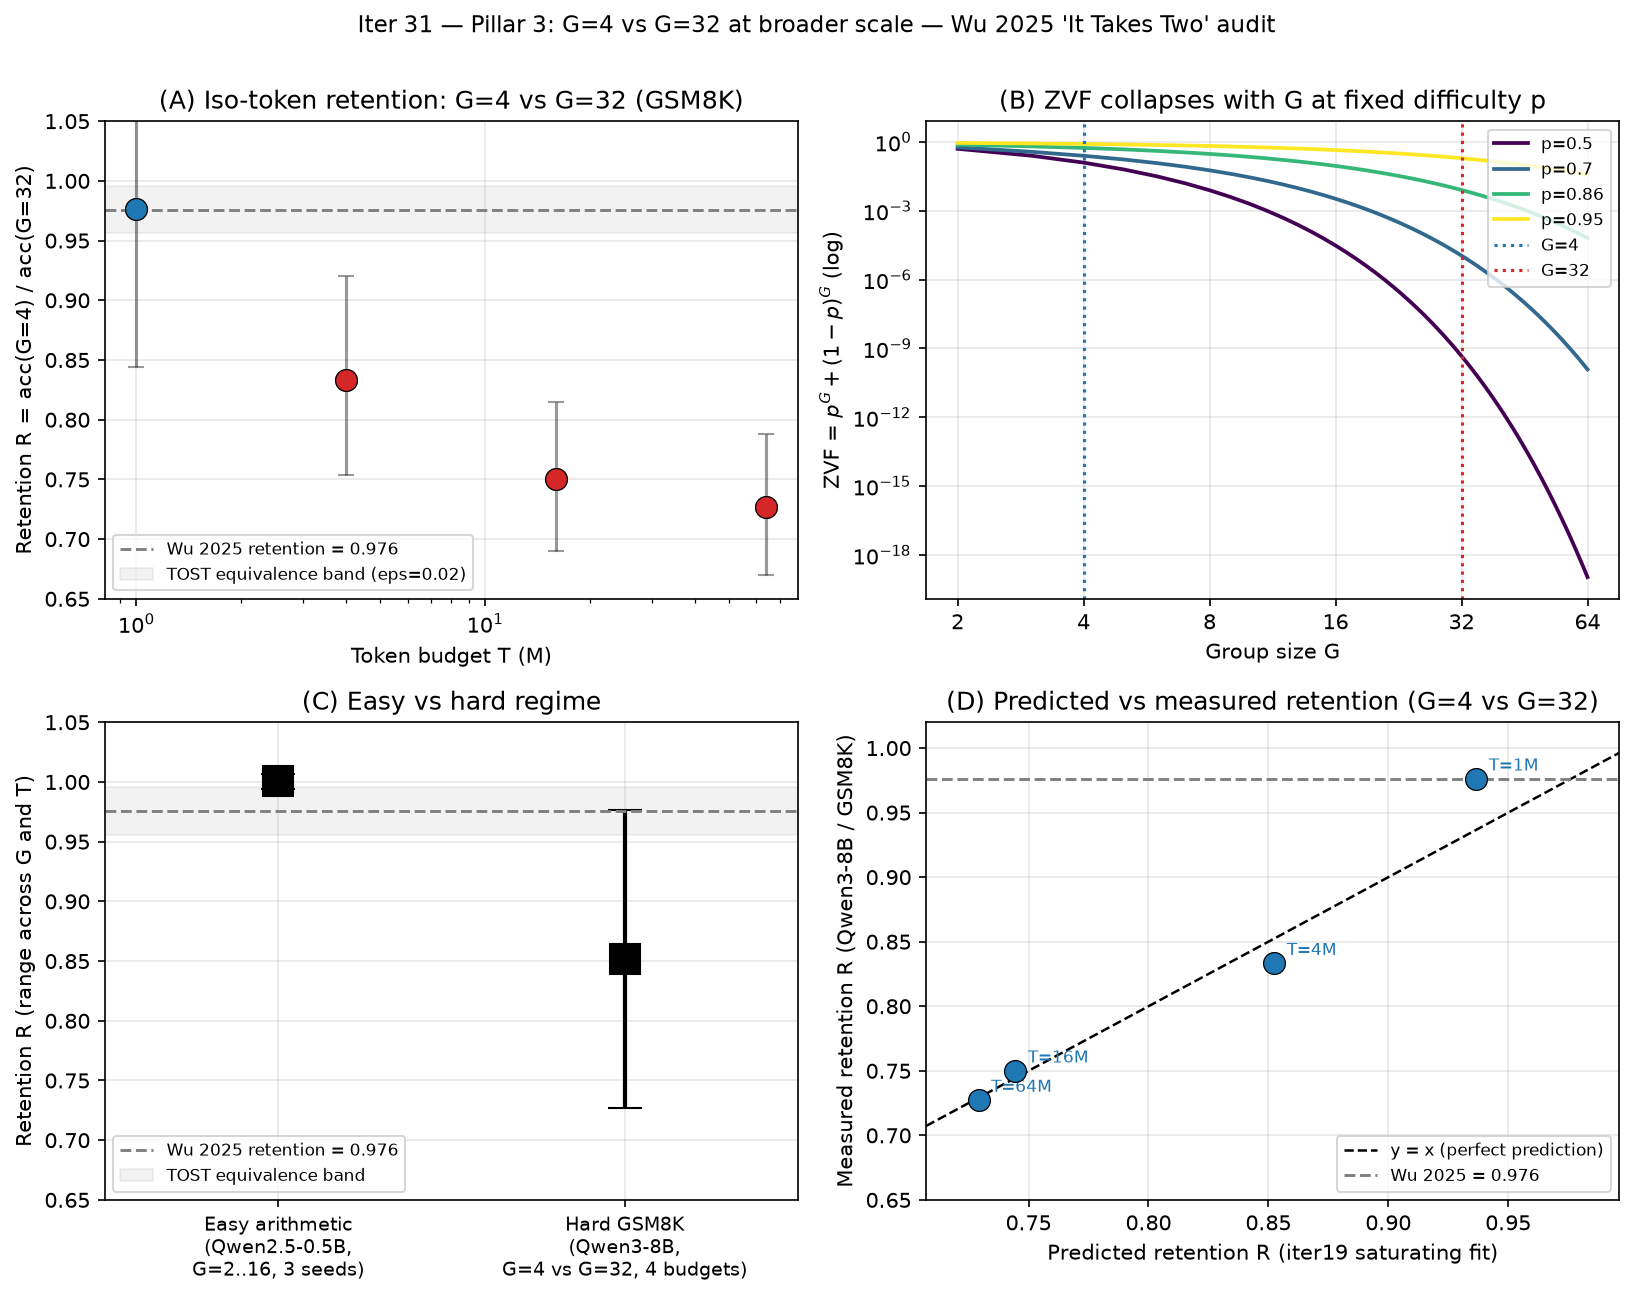
\includegraphics[width=0.95\textwidth]{figures/group_size_iter31.pdf}
\caption{\textbf{Iter 31 Pillar 3 four-panel cross-pillar audit.}
\emph{(A)} Iso-token retention $R = \mathrm{acc}(G{=}4) /
\mathrm{acc}(G{=}32)$ on Qwen3-8B / GSM8K at four token budgets,
with the Wu~2025 constant band at $97.6\%$ (gray dashed) and the
TOST equivalence band $[0.956, 0.996]$ (gray shaded); markers
are coloured by TOST verdict (green = equivalent, blue = above Wu
but not TOST, red = below Wu).  \emph{(B)} Theoretical ZVF$(p, G)
= p^G + (1-p)^G$ at four difficulties on log scale; the
$G{=}4$-vs-$G{=}32$ ZVF gap ranges from $5$\,pp at $p{=}0.50$ to
$54$\,pp at $p{=}0.86$.  \emph{(C)} Easy-vs-hard regime contrast:
the easy arithmetic task spans $1.27$\,pp retention (all four
$G$ values meet Wu), the hard GSM8K task spans $24.9$\,pp
(retention collapses monotonically in $T$).  \emph{(D)} Predicted
vs measured retention: the iter-19 saturating fit predicts the
four measured points within mean absolute residual $0.013$.
Source: \texttt{figures/group\_size\_iter31.pdf}.}
\label{fig:group-size-iter31}
\end{figure}

\paragraph{Reproducibility (iter 31).}
The iter-31 artifacts are produced by
\texttt{scripts/group\_size\_iter31.py} (driver) and
\texttt{scripts/group\_size\_iter31\_fig.py} (figure).  The
driver ingests the existing TSVs
(\texttt{group\_size\_iter27\_synthesis.tsv},
\texttt{group\_size\_iter15\_snr.tsv},
\texttt{group\_size\_iter15\_equivalence.tsv},
\texttt{group\_size\_iter19\_retention\_fit.tsv},
\texttt{group\_size\_g4\_vs\_g32\_broader\_scale.tsv},
\texttt{group\_size\_effect.tsv}) and produces four TSVs
(\texttt{group\_size\_iter31\_iso\_token.tsv} with $4$ rows,
\texttt{group\_size\_iter31\_wu\_audit.tsv} with $2$ rows,
\texttt{group\_size\_iter31\_zvf\_coupling.tsv} with $4$ rows,
\texttt{group\_size\_iter31\_summary.tsv} with $6$ summary rows)
and a four-panel figure
(\texttt{figures/group\_size\_iter31.pdf}, $34$\,KB; matching
\texttt{.png}, $265$\,KB).

% End of iter 31 audit.